\section * {Discussion} \label{sec:discuss}
The results concerning the simulated data were generally unsurprising. 
The more a phylogeny adheres to a molecular clock, the more accurate predictions made from it will be -- the simulated data is very well informed, and the phylogenies and their clocks are well resolved by the maximum likelihood tree estimate. 
Since latency is akin to ``pausing'' the evolution of a sequence, and evolution is assumed to be clock-like when sequences are not ``paused'', it's also not surprising that the latent simulated data could be reconstructed with low error. 

The results from the {\em plasma} data-set are also expected. 
Each patient from our plasma data-set showed evidence of a molecular clock, so the ability to reconstruct known dates came as no surprise. 
However, the reconstruction error was higher than that of the simulated data, which is expected for data that come from a real biological process.

Quantitatively, it's difficult to assess the accuracy of the reconstructions within the {\em mixed} data set. 
Many patients show evidence of latency in their regression plots (see the regression plot in Figure \ref{fig:results2} D) but it's unclear what the general pattern is (if any) for the distribution of the error metrics. 
Moreover, it's not possible to know the actual error for this data set, as that would require us to know the date at which a sequence became latent. 
We also observed an interesting sigmoidal pattern in many of the patients in this case.
However, we do note that most treated patients failed the hypothesis testing, implying that samples after treatment should be ignored in any analysis with this methodology.

Typically, we also observed that the rooting method had very little effect on the errors (the supplemental material has Figure \ref{fig:results2} replicated for RTT rooting). 
We did, however, identify a case in which RTT rooting fails over outgroup rooting (Figure \ref{fig:degenerate_example} shows an example of this). 
Specifically, it's possible for the calibration dates to provide insufficient data to resolve the root of the tree. 
We theorize that this is, for patient 820, because their calibration samples are strongly localized in time, which allows too much freedom (temporally) over the possible roots of the tree. 

%We did not attempt to use BEAST \citep{BEAST} to reconstruct any phylogenies from our data.
%Leaving dates unspecified on the number of tips would have drastically increased the dimensionality of the problem, and we would therefore need a prohibitively large amount of samples from the MCMC chain to assure convergence to the posterior distribution.

\begin{figure*}[!ht] \label{fig:degenerate_example}
	\centering
	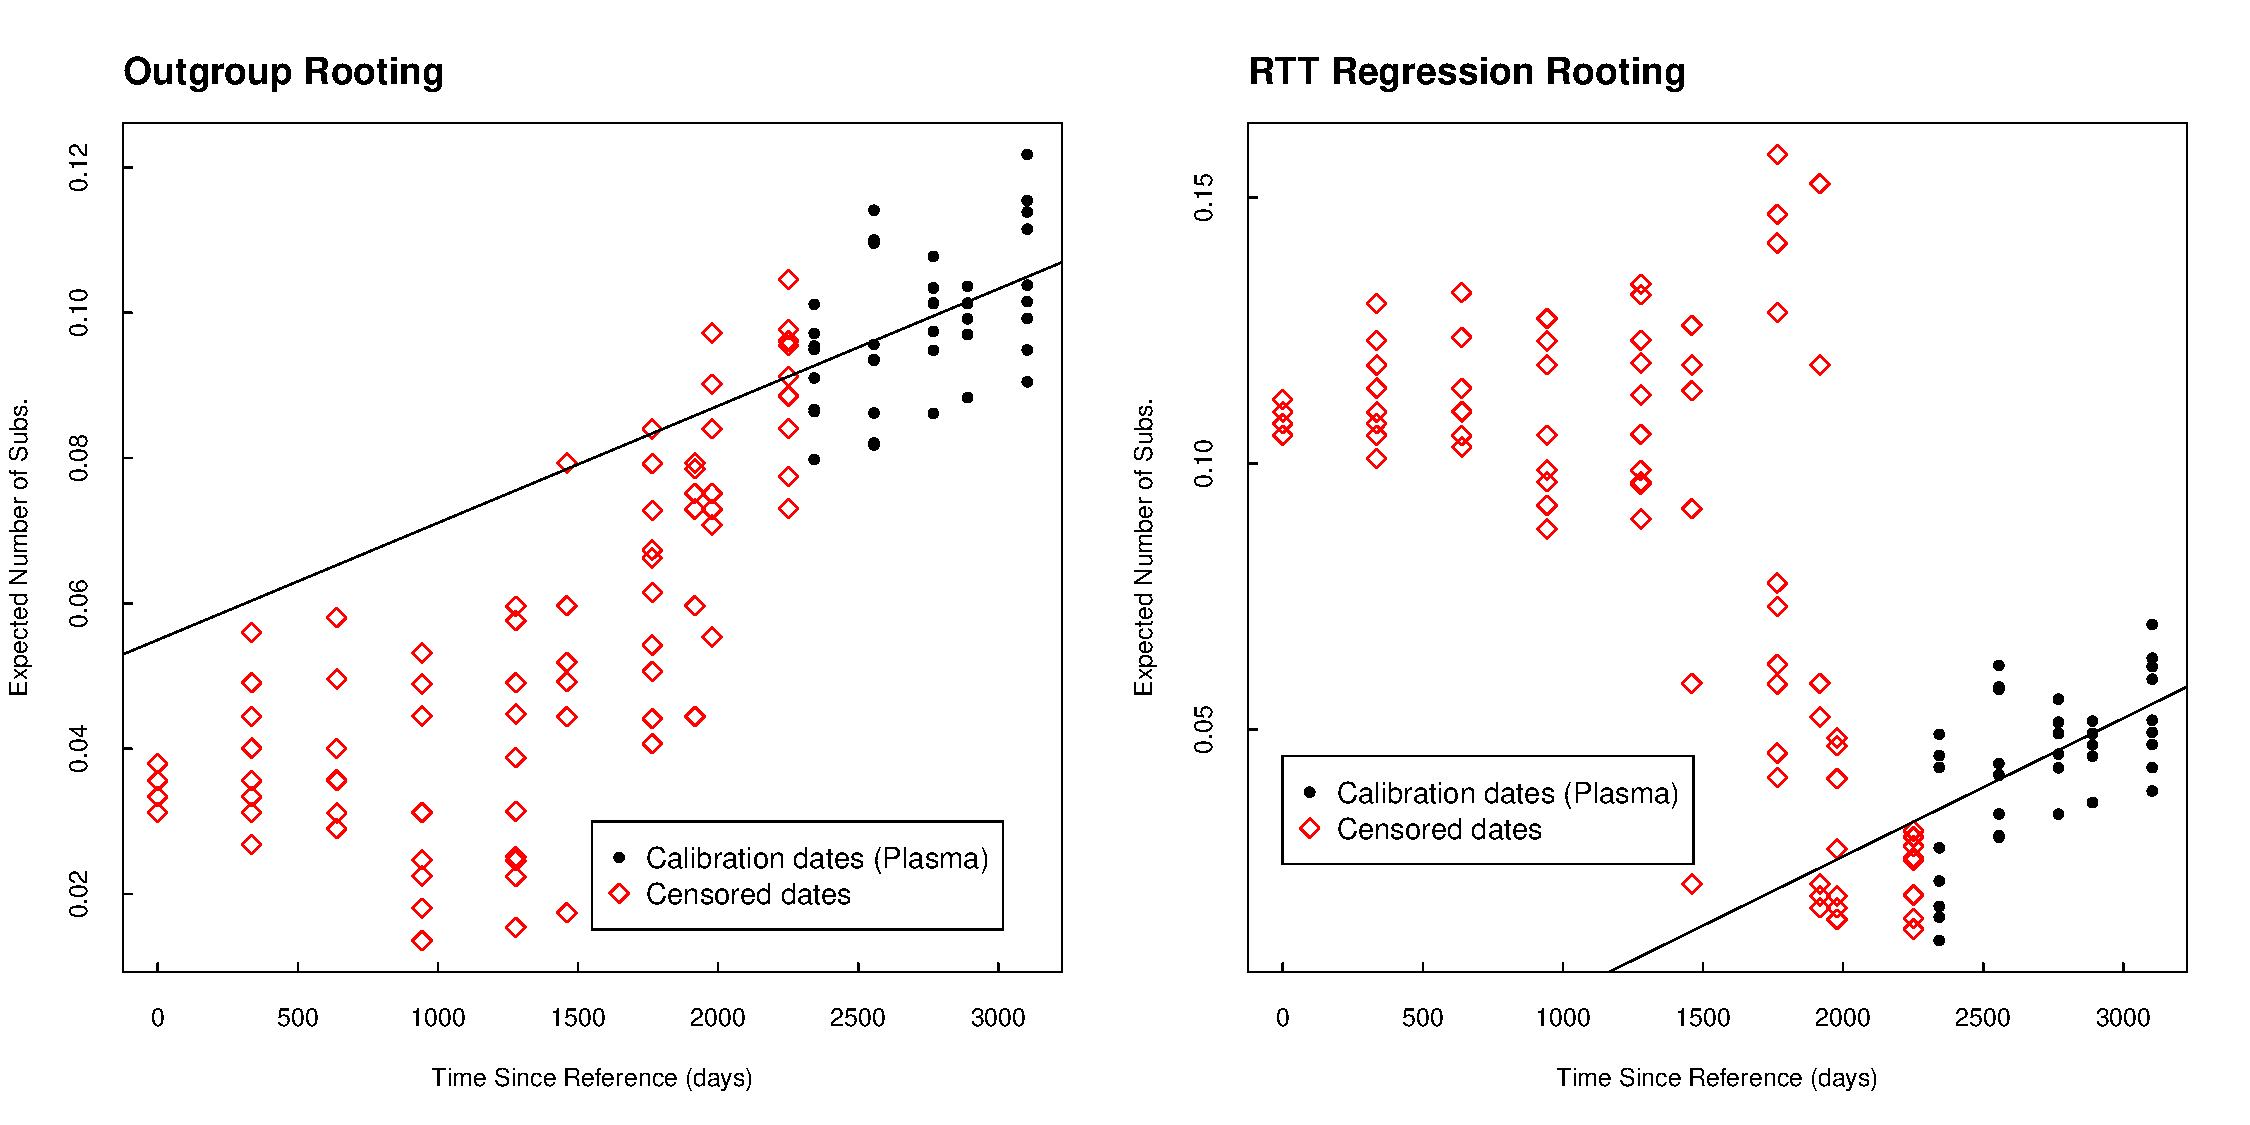
\includegraphics[scale=0.425]{figures/rtt.pdf} \\
	\caption[Example of bad root]{Root to tip rooting fails due to insufficient temporal resolution at the root}
\end{figure*}

We also noticed that the patients who had begun treatment (regardless of whether or not they regressed) typically failed the hypothesis testing. Upon analysing the clocks of these individuals, they showed two trends. 
The first trend, in patients who had regressed after treatment, was the ``resetting'' of the molecular clock -- that is, after treatment started, the clock was set to a previous point in time, then continued as it had before after treatment failed. 
For patients who had successfully been treated, there appeared to be an emergence of a clock with near zero slope after treatment.
This suggests that after a patient begins treatment, the assumption of a molecular clock  is not valid over the whole temporal range of the phylogeny. 


